\documentclass{article}
\usepackage[utf8]{inputenc}
\usepackage[english]{babel}
\usepackage{fullpage,amsmath,amssymb,graphics, graphicx,enumitem,ulem,parskip,xcolor,physics,csquotes,caption}

\usepackage[
backend=biber,
style=alphabetic,
sorting=ynt
]{biblatex}
\addbibresource{citations.bib}

\title{CSC311 Final Project}
\author{Jia Lin Yuan, Steven Tran, Luyang Shang}
\date{December 15, 2020}

\newcommand{\bs}{\boldsymbol}
\newcommand{\tbf}[1]{\textbf{#1}}
\newcommand{\mbf}[1]{\mathbf{#1}}
\newcommand{\mc}[1]{\mathcal{#1}}

\begin{document}
\maketitle
\section{Part A}
\begin{enumerate}[label=\arabic*.]
    \item For this approach, we use the KNN algorithm to impute the missing values.
        \begin{enumerate}[label=(\alph*)]
            \item See \texttt{knn.py} for the supporting code. For distance by user, we have:

                \noindent
                \begin{minipage}{0.5\linewidth}
                    \centering
                    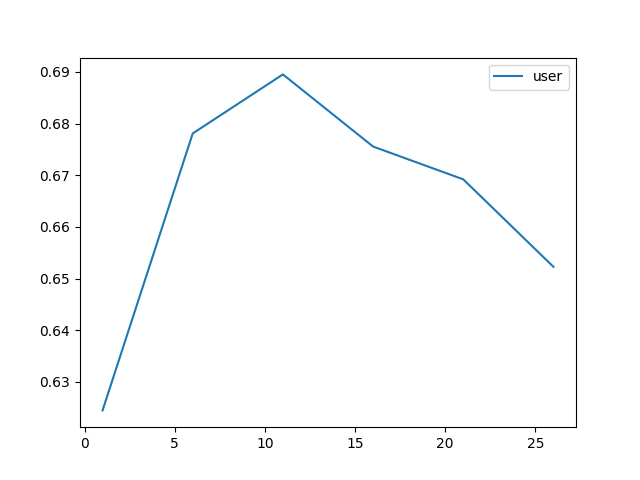
\includegraphics[width=\linewidth]{../starter_code/figs/knn_user.png}
                \end{minipage}\hfill
                \begin{minipage}{0.5\linewidth}
                    \center
                    \begin{tabular}{c|c}
                        $k$ & Validation Accuracy \\\hline
                        1 & 0.6244707874682472\\
                        6 & 0.6780976573525261\\
                        11 & 0.6895286480383855\\
                        16 & 0.6755574372001129\\
                        21 & 0.6692068868190799\\
                        26 & 0.6522720858029918
                    \end{tabular}
                \end{minipage}
            \item The best value of $k$ for user-based collaborative filtering is $k^*=11$.
            \item For distance by item, we have:

                \noindent
                \begin{minipage}{0.5\linewidth}
                    \centering
                    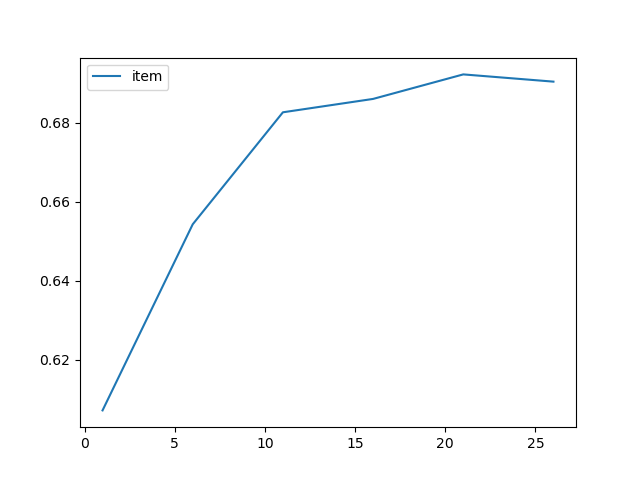
\includegraphics[width=\linewidth]{../starter_code/figs/knn_item.png}
                \end{minipage}\hfill
                \begin{minipage}{0.5\linewidth}
                    \center
                    \begin{tabular}{c|c}
                        $k$ & Validation Accuracy \\\hline
                        1 & 0.607112616426757\\
                        6 & 0.6542478125882021\\
                        11 & 0.6826136042901496\\
                        16 & 0.6860005644933672\\
                        21 & 0.6922099915325995\\
                        26 & 0.69037538808919
                    \end{tabular}
                \end{minipage}
                And the best value of $k$ for item-based collaborative filtering is $k^*=21$.
            \item For the chosen values of $k$: $k^*_{\text{user}}=11$, $k^*_{\text{item}}=21$, we find that the test accuracy is 0.68416596105 and 0.68165274090, respectively. So the user-based collaborative filtering performs better.
            \item Here are two limitations of KNN for this task:
                \begin{itemize}
                    \item KNN is slow. Even with only 542 items and 1774 users it takes a while to predict.
                    \item Using Euclidean distance, we consider distances in all dimension to be equal. For example if A and B's math skills are very different but english, physics, and other subjects are similar, the KNN will still predict A's math question similar to B's math questions (since skill in math is treated equally with other subjects).
                \end{itemize}

        \end{enumerate}
        
    \item In this approach, we use Item Response Theory to predict students' correctness to diagnostic questions.
        \begin{enumerate}[label=(\alph*)]
            \item Here, we derive an expression for the log-likelihood corresponding to this model and its derivative with respect to the user-ability and question-difficulty parameters. 
                \begin{align*}
                    \mc L(\mbf C|\bs\theta,\bs\beta) &= \sum_{i=1}^{N}{\sum_{j=1}^{J}{P(c_{ij}=1|\theta_i,\beta_j)^{c_{ij}}(1-P(c_{ij}=0|\theta_i,\beta_j))^{1-c_{ij}}}} \\
                    \ell(\mbf C|\bs\theta, \bs\beta) &= \sum_{i=1}^{N}{\sum_{j=1}^{J}{c_{ij}\log(P(c_{ij}=1|\theta_i,\beta_j))+(1-c_{ij})\log(1-P(c_{ij}=0|\theta_i,\beta_j))}} \\
                                                     &= \sum_{i=1}^{N}{\sum_{j=1}^{J}{\left(c_{ij}\left[(\theta_i-\beta_j)-\log(1+\exp(\theta_i-\beta_j))\right]+(1-c_{ij})\log \left(\frac{1}{1+\exp(\theta_i-\beta_j)}\right)\right)}} \\
                                                     &= \sum_{i=1}^{N}{\sum_{j=1}^{J}{\left(c_{ij}(\theta_i-\beta_j)-\log(1+\exp(\theta_i-\beta_j))\right)}} \\
                                                     &= \sum_{i\colon (i, j)\in C}{\sum_{j\colon (i, j)\in C}{\left(c_{ij}(\theta_i-\beta_j)-\log(1+\exp(\theta_i-\beta_j))\right)}} \\
                    \pdv{\ell}{\theta_i} &= \sum_{j\colon (i, j)\in C}{c_{ij}}-\sum_{j\colon (i, j)\in C}{\frac{\exp(\theta_i-\beta_j)}{1+\exp(\theta_i-\beta j)}} \\
                    \pdv{\ell}{\beta_j} &= \sum_{i\colon (i, j)\in C}{-c_{ij}} + \sum_{i\colon (i, j)\in C}{\frac{\exp(\theta_i-\beta_j)}{1+\exp(\theta_i-\beta j)}}
                \end{align*}
            \item We found the following hyperparameters to be the best:
                \begin{itemize}
                    \item learning rate=0.016
                    \item number of iterations=10 
                \end{itemize}
                Here is the plot of log-likelihoods on the training and validation data:
                \begin{center}
                    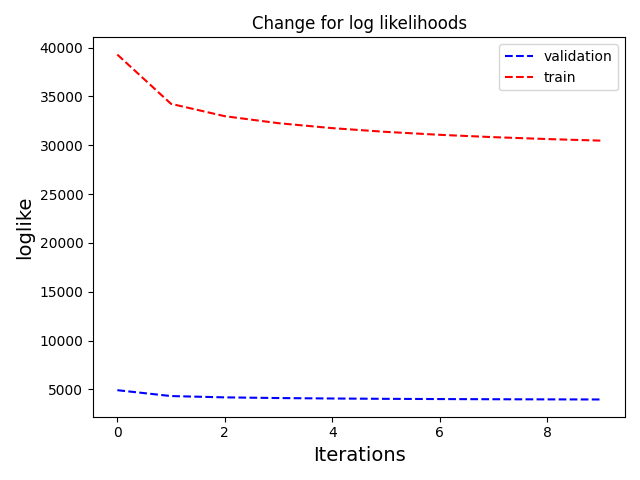
\includegraphics[width=0.6\linewidth]{../starter_code/irt_output/myplot.png}
                \end{center}
            \item For the same hyperparameters, we achieved:
                \begin{itemize}
                    \item Final validation accuracy: 0.7064634490544736
                    \item Final test accuracy: 0.7039232289020604
                \end{itemize}
            \item The plot is shown below. It shows the probability of correct response $P(c_{ij}|\theta_i,\beta_j)$ as a function of $\theta_i$, which represents the $i$-th student's ability. For each fixed question, the relationship between $P(c_{ij}|\theta_i,\beta_j)$ and $\theta$ follows the sigmoid function \[
                    P(c_{ij}|\theta_i,\beta_j)=\frac{\exp(\theta_i-\beta_j)}{1+\exp(\theta_i-\beta_j)}
            \] 
            There is a positive relationship between $P(c_{ij}|\theta_i,\beta_j)$ and $\theta$. It makes sense that a student having greater ability would be more likely to answer a question correctly if we hold the question difficulties constant.

            Also, notice that different questions have different correctness probabilities if we hold the students' abilities constant. For instance, the curve for the question with ID 3 is above the curve for the question with ID 4, indicating that the former is more likely to be correctly answered by students with equal ability compared to the latter question, which is comparatively harder.
                \begin{center}
                    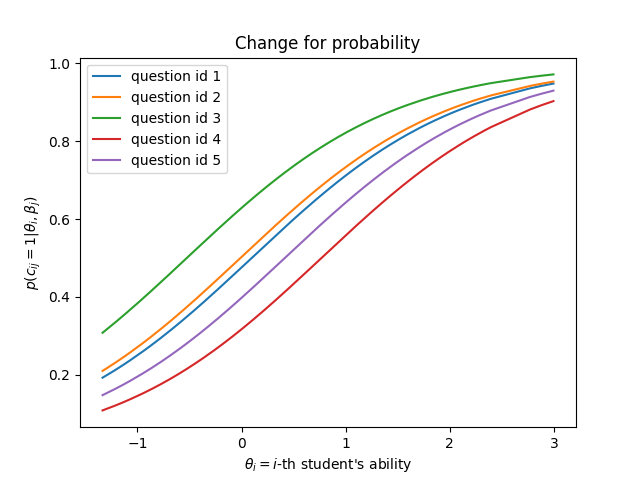
\includegraphics[width=0.6\linewidth]{../starter_code/figs/irt.png}
                \end{center}
        \end{enumerate}
        
    \item In this approach, we use neural networks. %both matrix factorization and neural networks.
        \begin{enumerate}[label=(\roman*)]
            \addtocounter{enumii}{1}
            %\item 
                %Matrix Factorization \textcolor{red}{remove this if we are not using it}
                %\begin{enumerate}[label=(\alph*)]
                %    \item d
                %\end{enumerate}
            \item Neural Networks
                \begin{enumerate}[label=(\alph*)]
                    \item \textcolor{red}{Not sure what this is asking.}
                    \item See \texttt{neural\_network.py}
                    \item We trained models using a variety of hyperparameters and found that a good combination was $k$ (latent dim.) = 10, learning rate = 0.01, epochs = 100. This achieved a training cost of 8376.565430	 and validation accuracy of 0.6891052780129834.
                    %\begin{center}
                    %    \begin{tabular}{c|c|c|c|c|c}
                    %        $k$ (latent dim.) & learning rate & epochs & $\lambda$ (penalty) & train cost & val. accuracy \\\hline
                    %        10 & 0.01 & 100 & 0.1 & 10545.283 & 0.68784 \\
                    %        10 & 0.01 & 100 & 0.5 & 19321.324219 & 0.69038 \\
                    %        50 & 0.05 & 10  & 0.5 & 17700.197 & 0.690799 \\
                    %        100 & 0.01 & 50 & 0.1 & 7667.879 & 0.68246 \\
                    %        100 & 0.05 & 10 & 0 & 6923.447 & 0.68346 \\
                    %        200 & 0.01 & 50 & 0.1 & 6638.1338 & 0.6782388 \\
                    %        200 & 0.01 & 50 & 0.5 & 16577.74 & 0.6745696 
                    %    \end{tabular}
                    %\end{center}
                    %Setting $k=500$ led to comparatively low validation accuracy (mean average of $0.651150$). For the other values of $k$, there weren't discernible correlations between the choice of hyperparameters and the performance of the model; the lower training cost and higher validation accuracy can probably be attributed to luck. We choose $k^*=10$ since the combination on the second row has a validation accuracy of 0.69038.
                    \item The final test accuracy was 0.6838837143663562.

                    \begin{center}
                        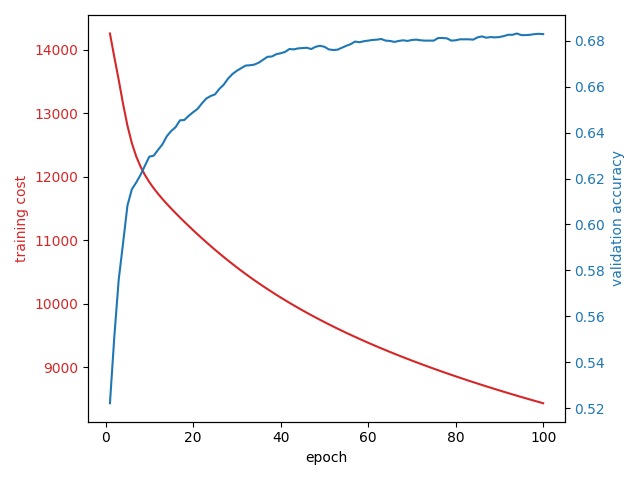
\includegraphics[width=0.6\linewidth]{../starter_code/nn_output/3d.png}
                    \end{center}
                \item We chose $\lambda=0.1$ and all of the other hyperparameters remain the same. This results in a final validation accuracy of 0.6830369743155518
and a test accuracy of 0.6850127011007621.

                    \begin{center}
                        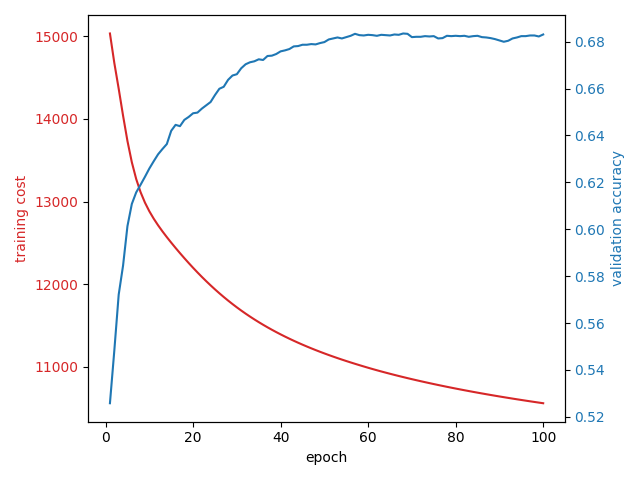
\includegraphics[width=0.6\linewidth]{../starter_code/nn_output/3e.png}
                    \end{center}
                \end{enumerate}
        \end{enumerate}
    \item For our ensemble, we decided to use the following base models:
        \begin{enumerate}
            \item Item response theory model with hyperparameters: 10 iterations, 0.016 learning rate
            \item ALS matrix factorization with hyperparameters: latent dimension 35, 0.01 learning rate, 500000 iterations
            \item Random-splitting decision tree with $\log_2n$ levels, i.e. it splits a node to be an internal node if there is at least 2 samples at that node.
        \end{enumerate}
        We also bootstrapped the training set by sampling three times with replacement, and then using one of those datasets for each of the models. The decisions of the three models are weighted equally, so the bagged model prediction was given by \[
            \frac{\sum_{d\in \text{data}}{\left(\text{pred}_{\text{IRT}}(d)+\text{pred}_{\text{ALS}}(d)+\text{pred}_{\text{tree}}(d)\right)}}{3}
        \] and then compared to the usual 0.5 threshold.

        The objective and reason why we employed this ensembling process was because we found it quite hard to push past the $\sim 0.68-0.70$ test accuracy threshold using only one base model without drastically overfitting on the training data. It was apparent through tuning of hyperparameters, especially for the neural network, that improvements may have been due to chance and that the models wouldn't generalize well to new data. In adding more predictors via bagging, we reduce the variance and reduce overfitting, but increase the bias. 

        The results of our implementation are as follows:
        \begin{itemize}
            \item Validation accuracy: 0.7039232289020604
            \item Test accuracy: 0.694609088343212
        \end{itemize}
\end{enumerate}

\newpage
\section{Part B}
\begin{enumerate}[label=\arabic*.]
    \item We chose to improve upon our matrix factorization model because our testing in Part A yielded the most promising results with this model on the test data. 

        We amended the initial squared error loss; the new objective function we aimed to minimize is \cite{netflix}: \[
            \mathcal{J}_{b\lambda} := \frac{1}{2}\sum_{(n, m)\in O}{\left(C_{nm}-\left(\mbf u_n^\top \mbf z_m+\mbf b_{u_n}+\mbf b_{z_m}+\mu\right)^2\right)+\lambda \left(\mbf u_n^\top\mbf u_n+\mbf z_m^\top\mbf z_m+\mbf b_{u_n}+\mbf b_{z_m}\right)}
        \] where:
        \begin{itemize}
            \item $\mbf b_{u_n}$ is a bias term for user $n$. It is initialized to the ratio of number of answers by user $n$ to the total amount of observed data, i.e. \[
                    \mbf b_{u_n} := \frac{\left|\left\{(n, m)\in O\right\}\right|}{\text{total observed data}}
            \] 
            \item $\mbf b_{z_m}$ is a bias term for question $m$. It is initialized to the ratio of number of answers for question $m$ to the total amount of observed data, i.e. \[
                    \mbf b_{z_m} := \frac{\left|\left\{(n, m)\in O\right\}\right|}{\text{total observed data}}
            \] 
            \item $\mu$ is a scalar initialized to the ratio of correct data to the total amount of observed data, i.e. \[
            \mu := \frac{\text{correct answers}}{\text{total observed data}}
            \] 
            \item $\lambda$ is a penalty/regularization term
        \end{itemize}

        We added weight regularization to the gradient descent method of optimizing the loss in our alternating least squares matrix factorization algorithm and bias/weight terms to every user and question. Intuitively, it is useful to weigh the users and questions that have more responses higher because they give more information, which is very useful when dealing with our issue of sparsity in the data. To start, given $k$, $\mbf u$ and $\mbf z$ were initialized by taking a uniform random sample of shape $(\text{\# user/question}, k)$ over $\left[0, \left\lfloor \frac{1}{\sqrt k}\right\rfloor\right]$. Then, we obtained the following update rules for $\operatornamewithlimits{argmin}_{\mbf u,\mbf z} \mathcal{J}_{b\lambda}$ via stochastic gradient descent:
        \begin{align*}
            \mbf u_n' &\gets \mbf u_n-\alpha \left(-\left(c_{nm}-\mu-\mbf b_{u_n}-\mbf b_{z_m}-\mbf u^\top\mbf z\right)\mbf z+\lambda\mbf u_n\right) \\
            \mbf z_m' &\gets \mbf z_m-\alpha \left(-\left(c_{nm}-\mu-\mbf b_{u_n}-\mbf b_{z_m}-\mbf u^\top\mbf z\right)\mbf u+\lambda\mbf z_m\right) \\
            \mbf b_{u_n}' &\gets \mbf b_{u_n}-\alpha \left(-(c_{nm}-\mu-\mbf b_{u_n}-\mbf b_{z_m}-\mbf u^\top\mbf z)+\lambda\mbf b_{u_n}\right) \\
            \mbf b_{z_m}' &\gets \mbf b_{z_m}-\alpha \left(-(c_{nm}-\mu-\mbf b_{u_n}-\mbf b_{z_m}-\mbf u^\top\mbf z)+\lambda\mbf b_{z_m}\right)
        \end{align*}
        Furthermore, we took this training approach for six models, each trained differently with corresponding $k$ values of $[40, 50, 60, 70, 80, 90]$. We did this in an attempt to reduce overfitting to the training data, reducing variance, and also increasing the bias. Their predictions were averaged and then compared to the usual threshold of 0.5, classifying the $(\text{user}, \text{question})$ pair as correct if it was greater. Another objective of this approach was to hopefully increase test performance by weighing more important points higher.
    \item In this section, we illustrate several ideas about our model. 

        \begin{minipage}[c]{0.35\linewidth}
            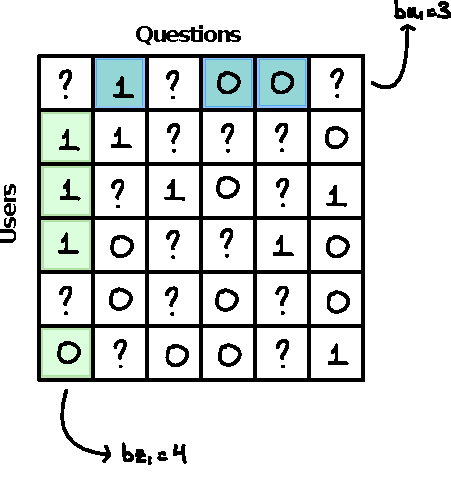
\includegraphics[width=\linewidth]{./images/train_sparse_bias.pdf}
            \captionof{figure}{Sparse train matrix showing how the user and question biases are initialized}
            \label{sparsebias}
        \end{minipage}\hfill
        \begin{minipage}[c]{0.6\linewidth}
            \begin{minipage}{0.4\linewidth}
                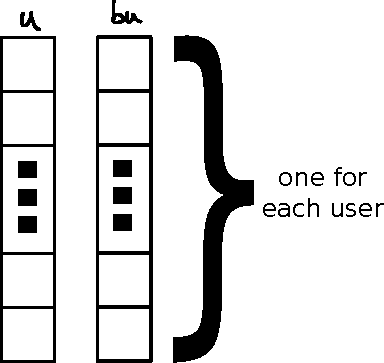
\includegraphics[width=\linewidth]{./images/bias_user.pdf}
            \end{minipage}\hfill
            \begin{minipage}{0.4\linewidth}
                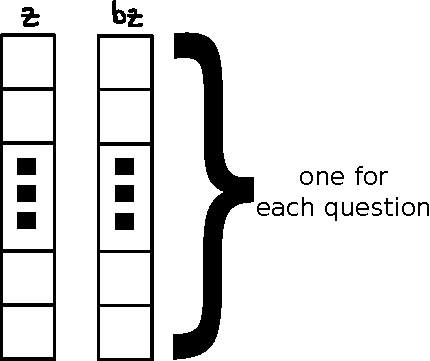
\includegraphics[width=\linewidth]{./images/bias_question.pdf}
            \end{minipage}
            \captionof{figure}{Parameters $\mbf u,\mbf z$ we aim to optimize for, and biases $\mbf b_u, \mbf b_z$}
            \label{biases}
        \end{minipage}

        Firstly, the model's goal is to take the training matrix in Figure~\ref{sparsebias} and complete it so that the unobserved entries, marked `?', are predicted. The $N\times J$ matrix can split into two matrices $\mbf u$ (size $N\times k$) and $\mbf z$ (size $J\times k$), where $k$ is the latent dimension hyperparameters, as shown in Figure~\ref{biases} for $k=1$. The reconstruction works by multiplying $\mbf u,\mbf z$:
        \[
            \underbrace{\mbf u}_{N\times k}\underbrace{\mbf z^\top}_{k\times J}=\underbrace{\text{reconstructed matrix}}_{N\times J}
        \] 
        For bootstrapping the training data, we sampled the indices of the training data with replacement so that duplicates would be included, meaning some points could be represented more than once. This is shown in Figure~\ref{bagging}.

        \begin{center}
            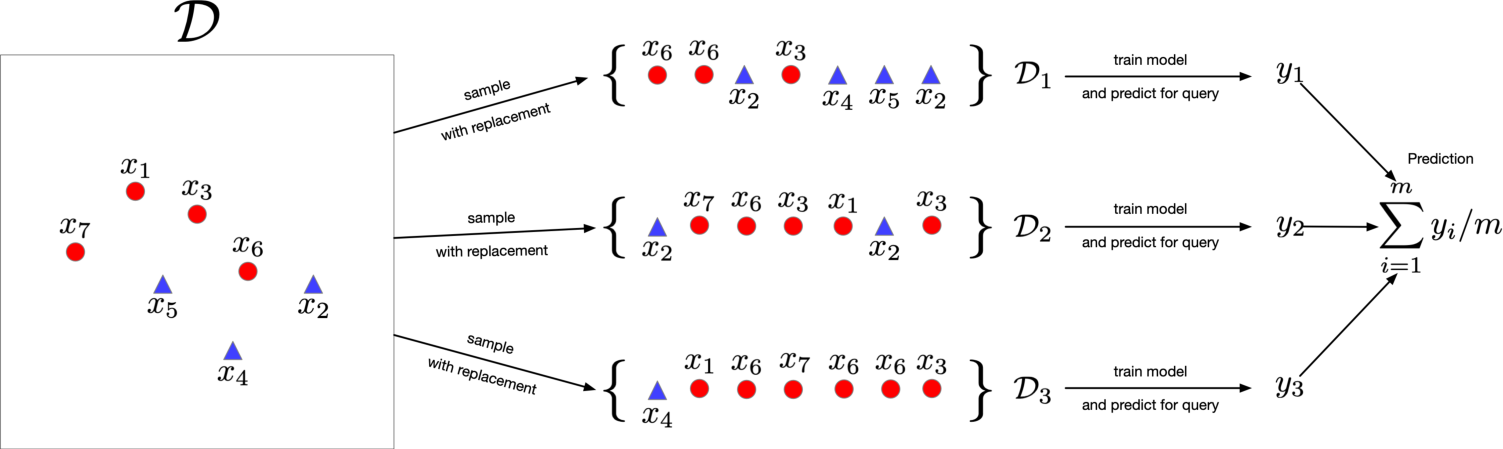
\includegraphics[width=\linewidth]{./images/bagging.pdf}
            \captionof{figure}{Illustration of bagging approach for the various matrix factorization models, taking the average of the predictions for the base models as the overall prediction~\cite{bagginglec}.}
            \label{bagging}
        \end{center}

    \item In this section, we compare the performance of our model using the same initialization of $\mbf u,\mbf z$, learning rate, and number of iterations with the baseline ALS matrix completion model. We will consider the training loss and prediction accuracy on the test data to see if our changes were useful.

        \begin{minipage}{0.49\linewidth}
            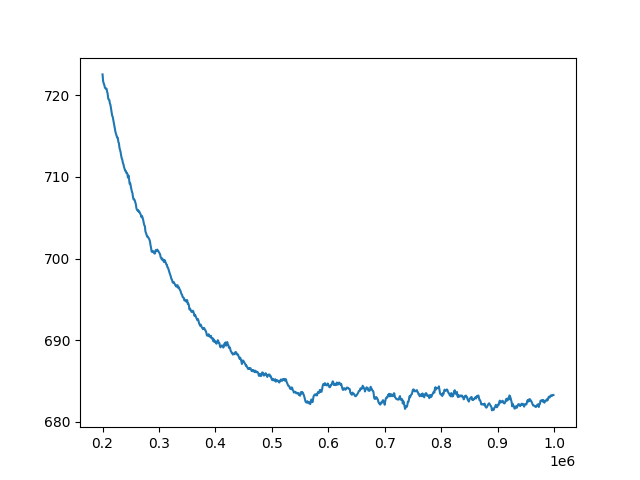
\includegraphics[width=\linewidth]{../starter_code/figs/sgd_wo_k_40.png}
            \captionof{figure}{$k=40$}
        \end{minipage}\hfill
        \begin{minipage}{0.49\linewidth}
            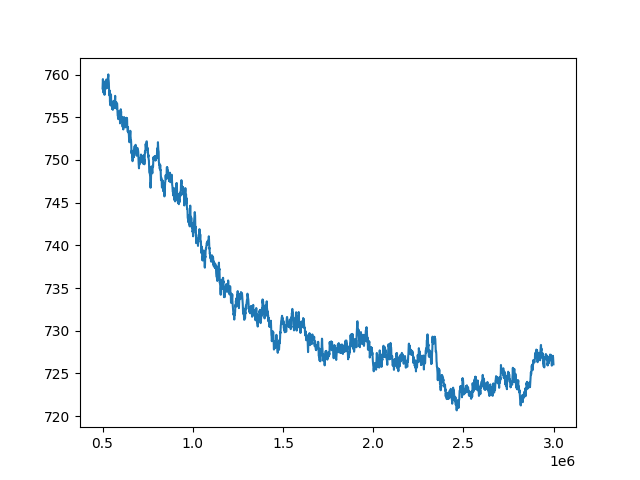
\includegraphics[width=\linewidth]{../starter_code/figs/sgd_k40.png}
            \captionof{figure}{$k=40$}
        \end{minipage}\hfill
        \begin{minipage}{0.49\linewidth}
            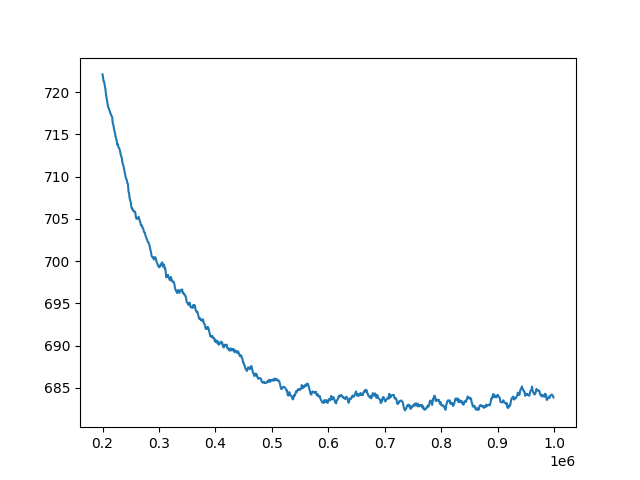
\includegraphics[width=\linewidth]{../starter_code/figs/sgd_wo_k_50.png}
            \captionof{figure}{$k=50$}
        \end{minipage}\hfill
        \begin{minipage}{0.49\linewidth}
            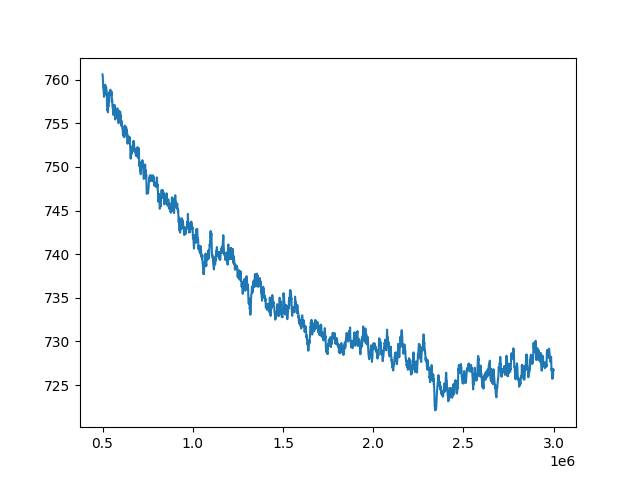
\includegraphics[width=\linewidth]{../starter_code/figs/sgd_k50.png}
            \captionof{figure}{$k=50$}
        \end{minipage}\hfill
        \begin{minipage}{0.49\linewidth}
            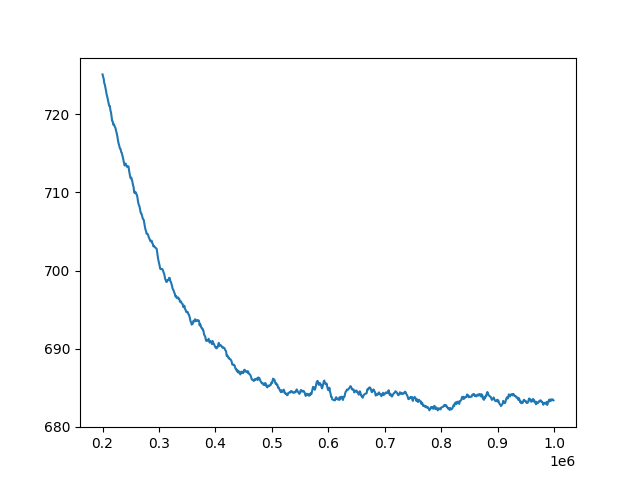
\includegraphics[width=\linewidth]{../starter_code/figs/sgd_wo_k_60.png}
            \captionof{figure}{$k=60$}
        \end{minipage}\hfill
        \begin{minipage}{0.49\linewidth}
            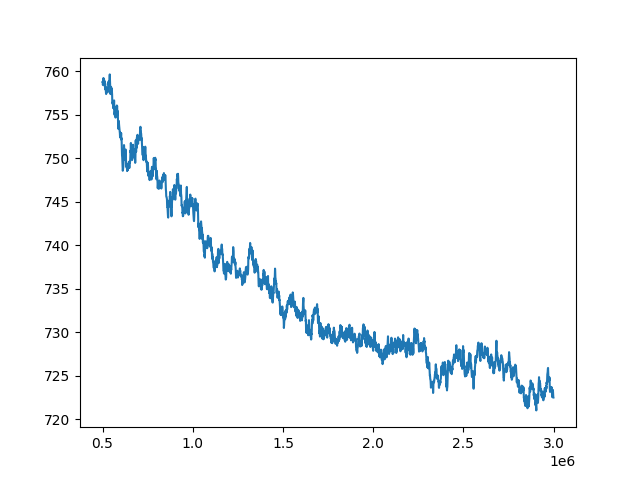
\includegraphics[width=\linewidth]{../starter_code/figs/sgd_k60.png}
            \captionof{figure}{$k=60$}
        \end{minipage}\hfill
        \begin{minipage}{0.49\linewidth}
            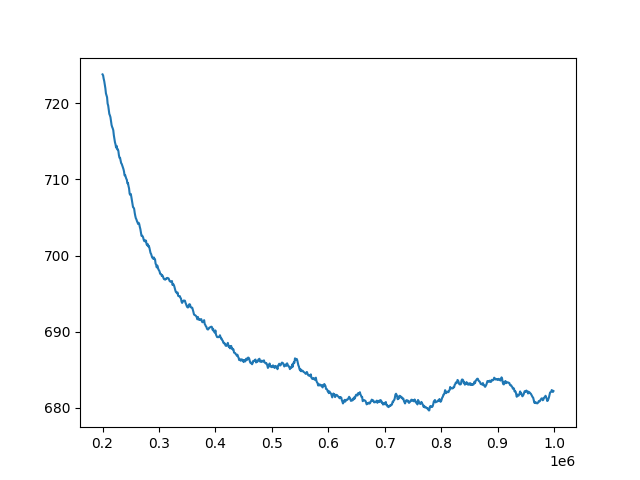
\includegraphics[width=\linewidth]{../starter_code/figs/sgd_wo_k_70.png}
            \captionof{figure}{$k=70$}
        \end{minipage}\hfill
        \begin{minipage}{0.49\linewidth}
            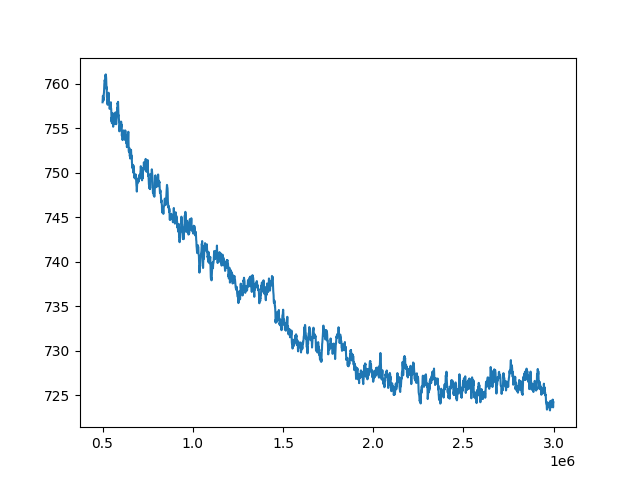
\includegraphics[width=\linewidth]{../starter_code/figs/sgd_k70.png}
            \captionof{figure}{$k=70$}
        \end{minipage}\hfill
        \begin{minipage}{0.49\linewidth}
            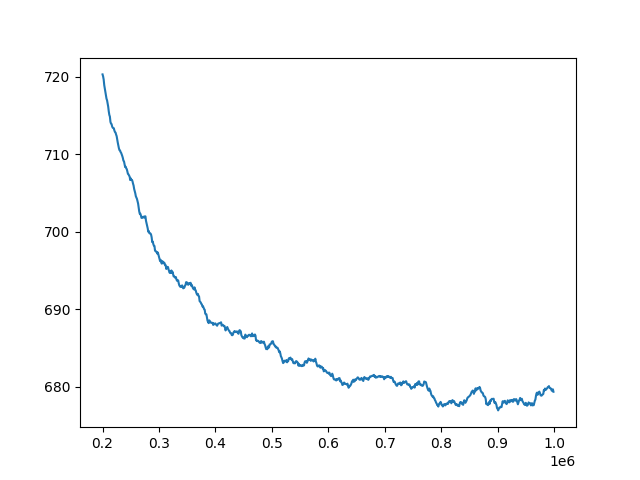
\includegraphics[width=\linewidth]{../starter_code/figs/sgd_wo_k_80.png}
            \captionof{figure}{$k=80$}
        \end{minipage}\hfill
        \begin{minipage}{0.49\linewidth}
            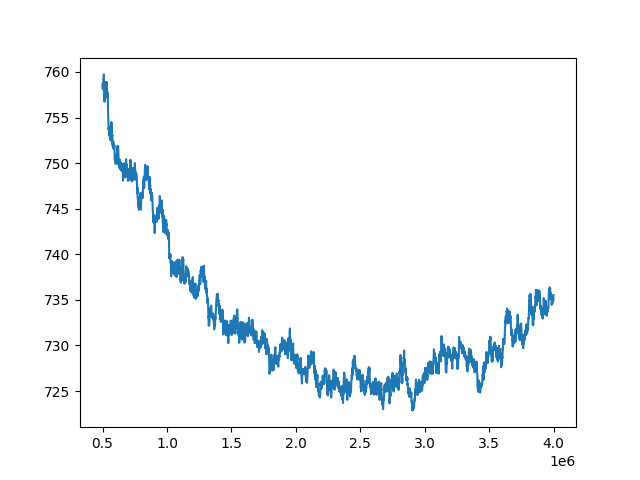
\includegraphics[width=\linewidth]{../starter_code/figs/sgd_k80.png}
            \captionof{figure}{$k=80$}
        \end{minipage}\hfill
        \begin{minipage}{0.49\linewidth}
            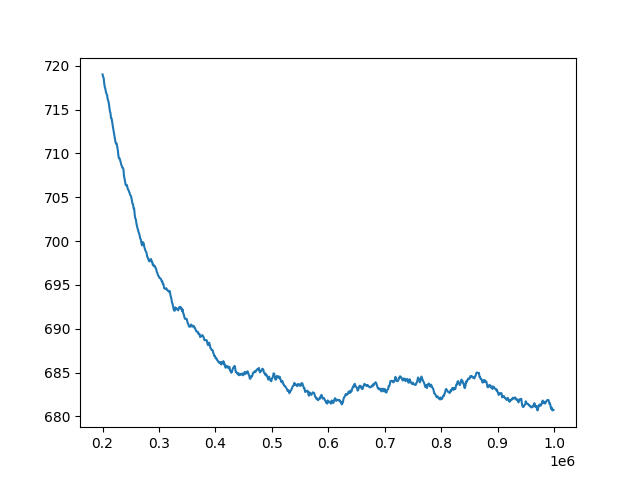
\includegraphics[width=\linewidth]{../starter_code/figs/sgd_wo_k_90.png}
            \captionof{figure}{$k=90$}
        \end{minipage}\hfill
        \begin{minipage}{0.49\linewidth}
            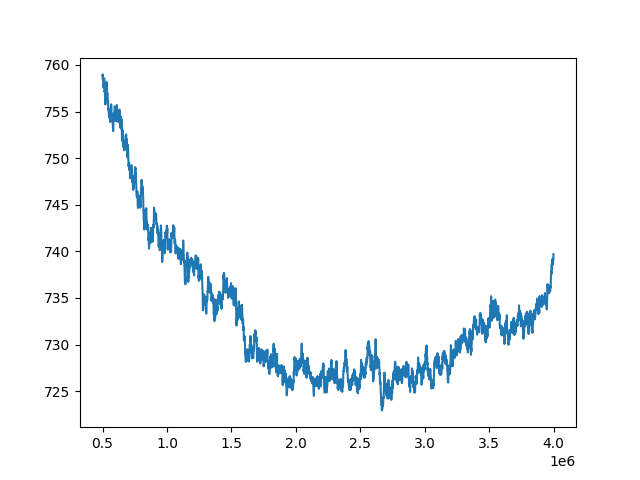
\includegraphics[width=\linewidth]{../starter_code/figs/sgd_k90.png}
            \captionof{figure}{$k=90$}
        \end{minipage}\hfill
    \item Our method may perform poorly if the weights are roughly equal, since there wouldn't be a gain in this instance. Another shortcoming is the lack of appropriate metadata that could help with weighing the features. We also don't have a lot of data to work with, and that's likely the reason why most models we have attain only around 70\% accuracy on the training, validation, and test sets. 
\end{enumerate}
\printbibliography[title={\section{References}}]
\end{document}
